\subsection{Game with incomplete information}
In this game we have included the problem of information asymmetry, this is done by letting nature selecting whether a player is insured or not, a player is insured with probability $p$, and not insured with probability $1-p$. 
The game is as described earlier in this chapter, link establishment is a bilateral decision, and we select two random nodes each round, and check if they would like to connect to each other. The difference is that we have inserted information asymmetry, only player 1 knows the type of the other player. Both players knows their own type, but player 2 only have a belief about the type of player 1.
\subsection{Calculating the different equlibriums}
In this game we have two types of players, type 1 $(t1)$: insured and type 2 $(t2)$: not insured. 
Player 1's type is chosen randomly by nature, with probability $p$ of being type 1 and $1-p$ of being type 2.
\begin{figure}[h]
\centering
  \centering
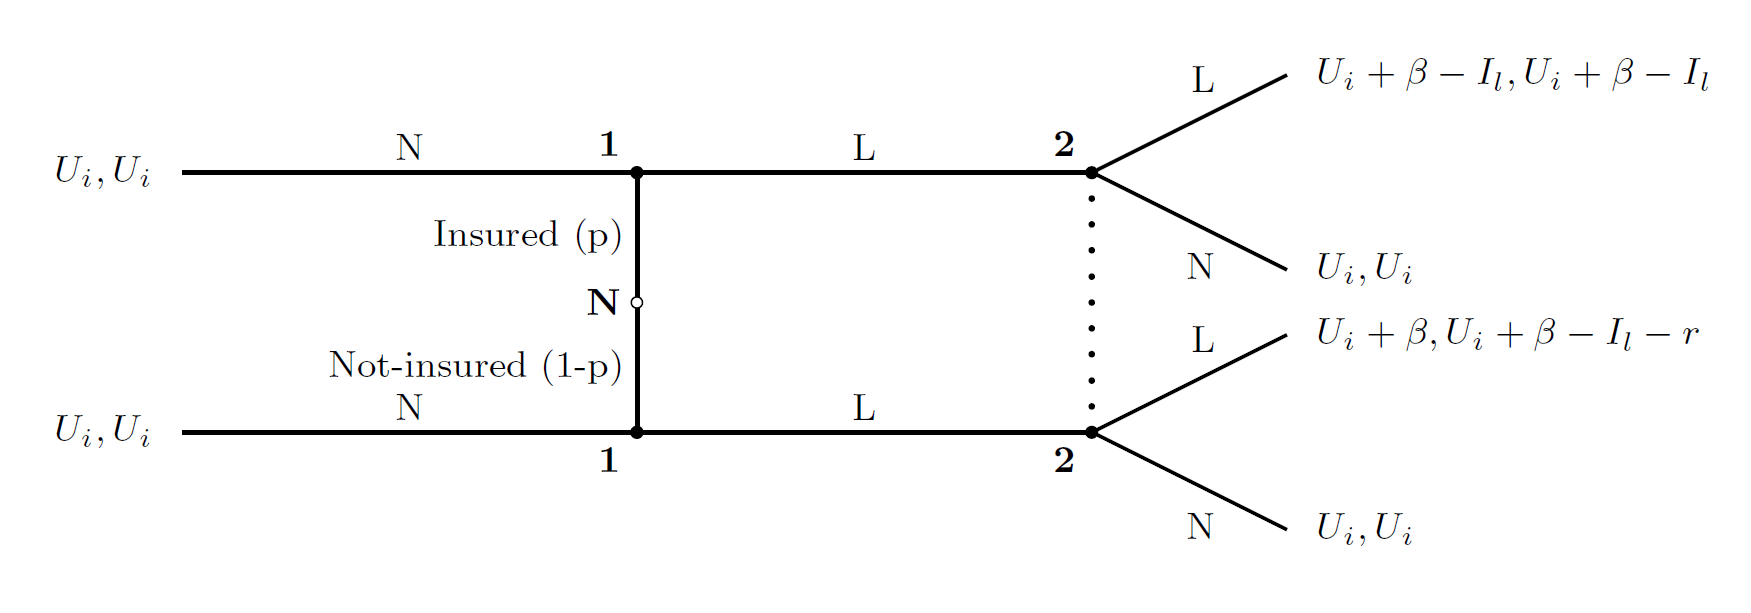
\includegraphics[width=1\linewidth]{../Figures/SignalingGameInsured.png}

\caption{Signalling game with two players, player 1's type choosen by nature, player2 is insured. Player 1 have complete information, player 2 suffer from incomplete information, and act on best response functions based on beliefs. \label{fig:signalingInsured}}

\end{figure}
In this two person game player 1 have complete information, i.e. he knows his own and the other players type. Player 2 suffer has incomplete information and only knows his own type. 
In the extensiveform shown in figure \ref{fig:signalingInsured}, we see that $t2's$ strategy L dominates N, and thus $t2$ will never play $N$.
\subparagraph{Separating equilibrium}
If we can find a separating equilibrium, this will enable player 2 to distinguish the two possible types of player 1.
Since player 1 will never play $N$ as type 2, there are only one possible separating equlibrium, type 1 plays $L$ and type 2 plays $N$. Hence player 2's beliefs are as in equation \ref{eq:player2belief}.
\begin{equation}
    \sigma_{1}(t_{i})= 
\begin{cases}
   N,& \text{if } t1\\
   L,& \text{if } t2  
\end{cases}
\label{eq:player2belief}
\end{equation}
Let $\mu_{1}(t_{i} | N )$, denote the probability that player 1 is of type $t_{i}$. And by using bayes rule we get this equation:
\begin{equation}
\mu_{1}(t_{1} | N )=\frac{P(N|t_{1})P(t_{1})}{P(N)}=\frac{P(N|t_{1})P(t_{1})}{P(N|t_{1})P(t_{1})+P(N|t_{2})P(t_{2})}
\end{equation}
And with player 2's belief, we get that $\mu_{1}(t_{1} | N )=1$ and $\mu_{1}(t_{2} | L )= 1 $. Now we calculate player 2's expected utility from playing L and N:
\begin{eqnarray}
EU_{2}(L,L)=\mu_{1}(t_{1} | L )U_{2}(L,L;t_{1})+\mu_{1}(t_{2} | L )U_{2}(L,L;t_{2}) \nonumber\\
\llap{$\rightarrow$\hspace{50pt}}EU_{2}(L,L)=U_{i}+\beta-I_{l}-r \\
EU_{2}(N,L)=\mu_{1}(t_{1} | L )U_{2}(N,L;t_{1})+\mu_{1}(t_{2} | L )U_{2}(N,L;t_{2})\nonumber\\
\llap{$\rightarrow$\hspace{50pt}}EU_{2}(N,L)=U_{i}
\end{eqnarray}
From these two equations we see that the best response of player 2($BR_2$) when he observes the other player choosing action $L$ is:
\begin{equation}
BR_{2}(L)=
\begin{cases}
L, & \text{if }\beta - r \geq I_{l}\\
N, & \text{if } \beta -r<I_{l}
\end{cases}
\label{eq:insuredBR}
\end{equation}
Player 2's expected utility when type 1 chooses N, is easily seen to be $U_{i}$. 
To confirm if this is a separating equilibrium we must see if player 1 has any incentive to deviate from the strategies in player 2's belief.
Type 2 will never deviate, so lets investigate type 1.
For player 1 to be willing to play N when he knows player 2's best response function, this must hold: $\beta<I_{l}$. If this is true, then player 2's best response is to play N. I.e. the only separating equilibrium is the following:

\begin{eqnarray}
\beta<I_{l}\\
 \sigma_{1}= 
\begin{cases}
   N,& \text{if } t1\\
   L,& \text{if } t2  
\end{cases}\\
BR_{2}(\sigma_{1})=N
\end{eqnarray} 
This means that in a separating equilibrium, the game will end up with no link establishment.
\subparagraph{Pooling equilibrium}
In a pooling equilibrium player 2 will not be able to distinguish the two types, and since $t1$'s strategy $L$ dominates $N$, i.e. there is only one possible equilibrium, the one where both types of player 1 plays $L$.
\begin{equation}
    \sigma_{1}(t_{i})= 
\begin{cases}
   L,& \text{if } t1\\
   L,& \text{if } t2  
\end{cases}
\label{eq:player2beliefpooling}
\end{equation}
By using bayes rule we get that $\mu(t_{1}|L)=p$ and $\mu(t_{2}|L)=1-p$.
Player 2's expected utility is then:
\begin{eqnarray}
EU_{2}(L,L)=p(U_{i}+\beta-I_{l})+(1-p)(U_{i}+\beta-I_{l}-r)\nonumber\\
\llap{$\rightarrow$\hspace{50pt}}EU_{2}(L,L)=U_{i}+\beta-I_{l}-r+r\\
EU_{2}(N,L)=U_{i}
\end{eqnarray}
From this we get player2's best response:
\begin{equation}
BR_{2}(L)=
\begin{cases}
L ,& \text{if } \beta + rp-r\geq I_{l} \\
N ,& \text{if } \beta +rp -r < I_{l} 
\end{cases}
\end{equation}
By using this best response function, player 1 sees that as long as $\beta>I_{l}$ he will never deviate from player 2's beliefs. And it is a pooling equilibrium where both player choose $L$, as long as $\beta>I_{l}$ and $\beta +rp-r>I_{l}$.
We also know that this: $rp-r<0$ is allways true, and thus there also exists a pooling equilibrium where player 1, plays $L$, and player 2, plays $N$. This will occur when $\beta>I_{l}$ and $\beta+rp-r<I_{l}$.
\subparagraph{Player 2 not insured, player 1's type choosen by nature}
The rules of the game are as before, the only thing that has changed is the type of player 2, and thus the payoffs are different and we need to see if there exists separating and pooling equilibrium in this game as well.
\begin{figure}[h]
\centering

  \centering
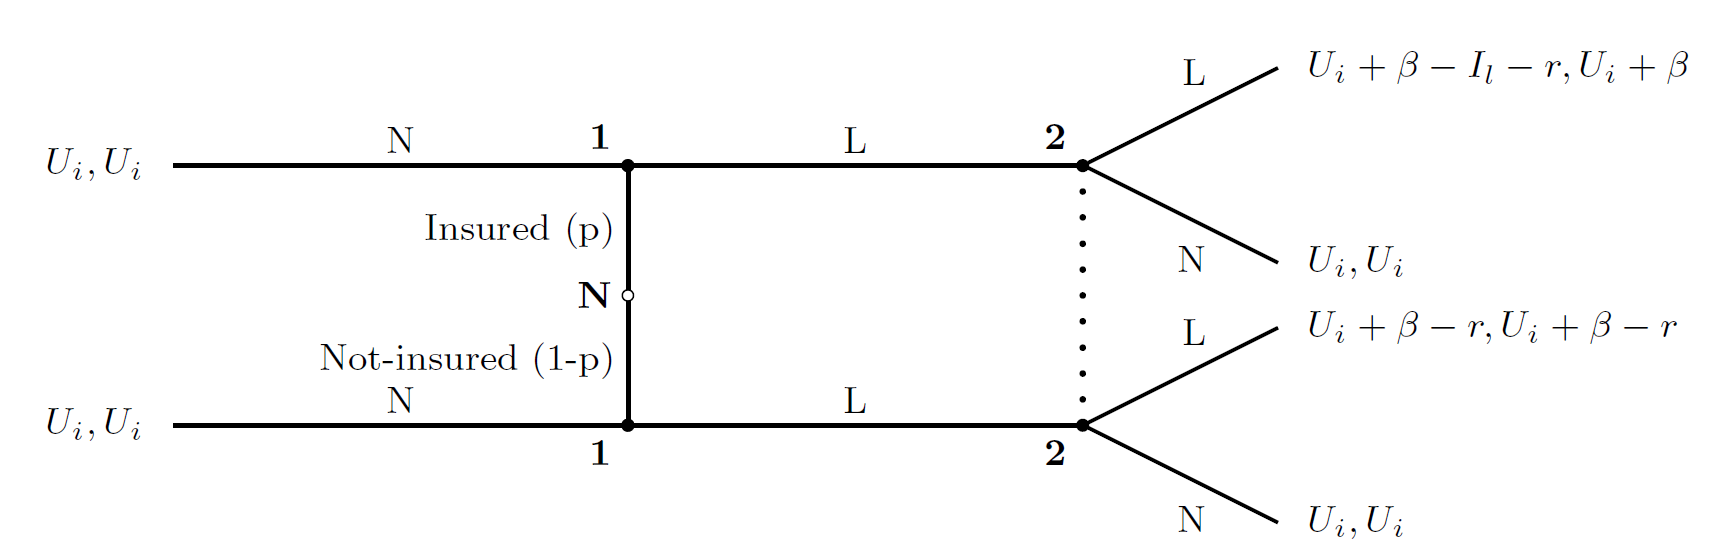
\includegraphics[width=1\linewidth]{../Figures/SignalingGameNotInsured.png}

\caption{Signalling game with two players, player 1's type choosen by nature, player2 is not insured. Player 1 have complete information, player 2 suffer from incomplete information, and act on best response functions based on beliefs. \label{fig:signalingNotInsured}}

\end{figure}
\subparagraph{Separating equilibrium}
In this game there is no dominant strategy for player 1, thus we have to check for the two possible separating equilibriums.
We start with the separating equilibrium with the beliefs shown in equation \ref{eq:player2beliefnotinsured}.
\begin{equation}
    \sigma_{1}(t_{i})= 
\begin{cases}
   L,& \text{if } t1\\
   N,& \text{if } t2  
\end{cases}
\label{eq:player2beliefnotinsured}
\end{equation}
With the beliefs in equation \ref{eq:player2beliefnotinsured}, this is his expected payoffs:
\begin{eqnarray}
EU_{2}(L,L)=(U_{i}+\beta) \\
EU_{2}(N,L)=(U_{i})
\end{eqnarray}
From this we see that his best response when player 1's action is L, is to allways play $L$: \begin{equation}
BR_{2}(L)= L
\end{equation}
To see if this is an equilibrium, we have to see if player 1 has any incentive to deviate. 
Lets check for the two types of player 1:
If $\beta>r$ then type 2 would deviate, because he could achieve a higher payoff by playing $L$, given the beliefs of player 2 in equation \ref{eq:player2beliefnotinsured}. So we know that for this to be an equilibrium, \begin{equation}
\beta < r
\label{eq:sepcondition}
\end{equation}  
When analyzing from player 1 type 1's perspective, for him to play L, this has to hold: $U_{i}+\beta-I_{l}-r > U_{i}$. The only way this can hold is if $\beta>I_{l}+r$. We see that equation \ref{eq:sepcondition} is violating this condition, and thus we have no separating equilibrium with the beliefs in equation \ref{eq:player2beliefnotinsured}.
Now lets look at the other possible separating equilibrium, see equation \ref{eq:player2beliefnotinsured2}.
\begin{equation}
    \sigma_{1}(t_{i})= 
\begin{cases}
   N,& \text{if } t1\\
   L,& \text{if } t2  
\end{cases}
\label{eq:player2beliefnotinsured2}
\end{equation}
Player 2's expected payoffs are as follows:
\begin{eqnarray}
EU_{2}(L,L)=U_{i}+\beta-r \\
EU_{2}(N,L)=U_{i}
\end{eqnarray}
From this we get the best response function:
\begin{equation}
BR_{2}(L)=
\begin{cases}
L ,& \text{if } \beta\geq r \\
N ,& \text{if } \beta<r 
\end{cases}
\end{equation}
For this to be a separating equilibrium, we need to see if player 1 would deviate from player 2's beliefs. 
Type $t1$ will not deviate as long as $\beta<I_{l}+r$. Type $t2$ will not deviate if $\beta \geq r$, if this condition is true, we see that player 2 will play $L$. I.e. the only separating equilibrium that exists is when player 2 plays $L$, player 1 of type $t1$ plays $N$ and player 1 of type$t2$ plays $L$.
And for this to happen we get this condition on $\beta$. \begin{equation}
I_{l}+r>\beta>r
\label{eq:conditionseparatingequilibrium}
\end{equation}
\subparagraph{Pooling equilibrium}
Two possible, one where both types of player 1 plays $L$, and one where both types plays $N$. Lets first analyze the one where both types of player 1 plays $L$.
\begin{equation}
    \sigma_{1}(t_{i})= 
\begin{cases}
   L,& \text{if } t1\\
   L,& \text{if } t2  
\end{cases}
\label{eq:player2beliefnotinsuredpooling}
\end{equation}
With the beliefs shown above, player 2's expected payoffs are: \begin{eqnarray}
EU_{2}(L)=p(U_{i}+\beta)+(1-p)(U_{i}+\beta-r) \nonumber \\
EU_{2}(L)=U_{i}+\beta-r+pr \\
EU_{2}(N)=U_{i}
\end{eqnarray}
From this we get the best response function :
\begin{equation}
BR_{2}(L)=
\begin{cases}
	L,& \text{if } \beta\geq r-pr\\
   N,& \text{if } \beta<r-pr  
\end{cases}
\end{equation}
Will player 1 deviate knowing this?
Type $t1$ will not deviate as long as: $\beta - I_{l} \geq r$. And type $t2$ will not deviate as long as $\beta >r$.
From this we get this final condition, if $\beta-I_{l}\geq r$ then there exists a pooling equilibrium where both types of player 1 plays $L$ and player 2 also play $L$.
From this we can also see that the other pooling equilibrium where both types of player 1, plays $N$, can only happen when $\beta<r \text{ and } \beta<I_l+r$.

\subparagraph{Summary}
When the game is suffering from incomplete information, we are not able to ensure that the network formation game end up in an insurable clique. We found one equilibrium where the non-insured player 2 where able to separate the two types of player 1, and when $\beta>r+I_{l}$ the resulting network will be a clique of only non-insured nodes.
We also found pooling equilibriums where both types of player 1 and player 2 will connect to both non-insured and insured nodes. 
